\documentclass{ansarticle-preprint}
%\usepackage{ucs}
\usepackage[utf8]{inputenc}
\usepackage{amsmath}
%\usepackage{cite}
\usepackage{anslistings}
\usepackage{multicol}
\usepackage{pdfsync}
\usepackage{enumitem}

\usepackage{pgfplots}
\usepackage{pgfplotstable}

\usepackage{fontenc}
\usepackage{graphicx}
\usepackage{xspace}

\usepackage{siunitx}

\usepackage{floatflt}

\usepackage{multirow}

\usepackage{booktabs}

%\renewcommand{\baselinestretch}{2.0}
%\usepackage{lineno}
%\renewcommand\linenumberfont{\normalfont\tiny}
%\linenumbers	

\graphicspath{{svg/}}

\usepackage[normalem]{ulem}

\usepackage{caption}
\usepackage{subcaption}

\usepackage{todonotes}

\pgfplotsset{compat=1.9}
\definecolor{gnuplot@lightblue}{RGB}{87,181,232}
\definecolor{gnuplot@green}{RGB}{0,158,115}
\definecolor{gnuplot@purple}{RGB}{148,0,212}

\newcommand{\specialword}[1]{\texttt{#1}}
\newcommand{\dealii}{{\specialword{deal.II}}\xspace}
\newcommand{\pfrst}{{\specialword{p4est}}\xspace}
\newcommand{\trilinos}{{\specialword{Trilinos}}\xspace}
\newcommand{\aspect}{\specialword{Aspect}\xspace}
\newcommand{\petsc}{\specialword{PETSc}\xspace}
\newcommand{\snes}{{\specialword{SNES}}\xspace}
\newcommand{\ts}{{\specialword{TS}}\xspace}
\newcommand{\petscsf}{{\specialword{SF}}\xspace}
\newcommand{\cmake}{{\specialword{CMake}}\xspace}
\newcommand{\candi}{{\specialword{candi}}\xspace}
\newcommand{\sundials}{{\specialword{SUNDIALS}}\xspace}
\newcommand{\kinsol}{{\specialword{KINSOL}}\xspace}
\newcommand{\ida}{{\specialword{IDA}}\xspace}
\newcommand{\arkode}{{\specialword{ARKODE}}\xspace}


\usetikzlibrary{shapes.misc}
\tikzset{cross/.style={cross out, draw=black, minimum size=2*(#1-\pgflinewidth), inner sep=0pt, outer sep=0pt},
%default radius will be 1pt.
cross/.default={2pt}}

%
% Author list -- please add yourself in both places below (in
%                alphabetical order) if you think that your
%                contributions to the last release warrant this
%

\hypersetup{
  pdfauthor={
    Daniel Arndt,
    Wolfgang Bangerth,
    Maximilian Bergbauer,
    Marc Fehling,
    Marco Feder,
    Johannes Heinz,
    Timo Heister,
    Luca Heltai,
    Martin Kronbichler,
    Matthias Maier,
    Peter Munch,
    Jean-Paul Pelteret,
    Bruno Turcksin,
    David Wells,
    Stefano Zampini
  },
  pdftitle={The deal.II Library, Version 9.5, 2023},
}

\title{The \dealii Library, Version 9.5}

 \author[1*]{Daniel Arndt}
 \affil[1]{Computational Coupled Physics Group,
   Computational Sciences and Engineering Division,
   Oak Ridge National Laboratory, 1 Bethel Valley Rd.,
   TN 37831, USA.
   \texttt{arndtd/turcksinbr@ornl.gov}}

 \author[2,3]{Wolfgang~Bangerth}
 \affil[2]{Department of Mathematics, Colorado State University, Fort
   Collins, CO 80523-1874, USA.
   \texttt{bangerth/marc.fehling@colostate.edu}}
 \affil[3]{Department of Geosciences, Colorado State University, Fort
   Collins, CO 80523, USA.}

\author[4]{Maximilian~Bergbauer}
\affil[4]{Institute for Computational Mechanics,
Technical University of Munich,
Boltzmannstr.~15, 85748 Garching, Germany.
{\texttt{maximilian.bergbauer@tum.de}}}

\author[2]{Marc~Fehling}

\author[5]{Marco~Feder}
\affil[5]{SISSA,
International School for Advanced Studies,
Via Bonomea 265,
34136, Trieste, Italy.
{\texttt{marco.feder/luca.heltai@sissa.it}}}

\author[6]{Johannes~Heinz}
 \affil[6]{Institute of Mechanics and Mechatronics,
   TU Wien,
   Getreidemarkt 9, 1060 Vienna, Austria
   {\texttt{johannes.heinz@tuwien.ac.at}}}

\author[7]{Timo~Heister}
 \affil[7]{School of Mathematical and Statistical Sciences,
   Clemson University,
   Clemson, SC, 29634, USA
   {\texttt{heister@clemson.edu}}}

\author[5]{Luca~Heltai}

 \author[8]{Martin~Kronbichler}
 \affil[8]{Institute of Mathematics,
   University of Augsburg,
   Universit\"atsstr.~12a, 86159 Augsburg, Germany.
   {\texttt{martin.kronbichler/peter.muench@uni-a.de}}}

\author[9]{Matthias~Maier}
\affil[9]{Department of Mathematics,
  Texas A\&M University,
  3368 TAMU,
  College Station, TX 77845, USA.
  {\texttt{maier@math.tamu.edu}}}

\author[8,10]{Peter Munch}
 \affil[10]{Institute of Material Systems Modeling,
 Helmholtz-Zentrum Hereon,
 Max-Planck-Str. 1, 21502 Geesthacht, Germany}


\author[11]{Jean-Paul~Pelteret}
\affil[11]{Independent researcher.
{\texttt{jppelteret@gmail.com}}}

\author[1*]{Bruno~Turcksin}

\author[12]{David Wells}
\affil[12]{Department of Mathematics, University of North Carolina,
  Chapel Hill, NC 27516, USA.
  {\texttt{drwells@email.unc.edu}}}

\author[13]{Stefano Zampini}
\affil[13]{Extreme Computing Research Center, King Abdullah University of Science and Technology,
  23955-6900 Thuwal, Saudi Arabia.
  {\texttt{stefano.zampini@gmail.com}}}

\renewcommand{\labelitemi}{--}


\begin{document}
\maketitle

\footnotetext{%
  $^\ast$ This manuscript has been authored by UT-Battelle, LLC under Contract No.
  DE-AC05-00OR22725 with the U.S. Department of Energy.
  % We need to submit the manuscript with the text below. If the editor
  % complains we can remove it. 
  The United States
  Government retains and the publisher, by accepting the article for
  publication, acknowledges that the United States Government retains a
  non-exclusive, paid-up, irrevocable, worldwide license to publish or reproduce
  the published form of this manuscript, or allow others to do so, for United
  States Government purposes. The Department of Energy will provide public
  access to these results of federally sponsored research in accordance with the
  DOE Public Access Plan (http://energy.gov/downloads/doe-public-access-plan).
}


\begin{abstract}
  This paper provides an overview of the new features of the finite element
  library \dealii, version 9.5.
\end{abstract}



%%%%%%%%%%%%%%%%%%%%%%%%%%%%%%%%%%%%%%%%%%%%%%%%%%%%%%%%%%%%%%%%%%%%%%%%%%%%%%%%
%%%%%%%%%%%%%%%%%%%%%%%%%%%%%%%%%%%%%%%%%%%%%%%%%%%%%%%%%%%%%%%%%%%%%%%%%%%%%%%%
%%%%%%%%%%%%%%%%%%%%%%%%%%%%%%%%%%%%%%%%%%%%%%%%%%%%%%%%%%%%%%%%%%%%%%%%%%%%%%%%
\section{Overview}

\dealii version 9.5.0 was released XX XX, 2023.
This paper provides an
overview of the new features of this release and serves as a citable
reference for the \dealii software library version 9.5. \dealii is an
object-oriented finite element library used around the world in the
development of finite element solvers. It is available for free under the
GNU Lesser General Public License (LGPL). Downloads are available at
\url{https://www.dealii.org/} and \url{https://github.com/dealii/dealii}.

The major changes of this release are:
%
\begin{itemize}
  \item Substantial updates and extensions to \dealii{}'s interfaces
    to other libraries (see Section~\ref{sec:external}). This
    includes, in particular, the integration of \texttt{Kokkos} (Section~\ref{sec:kokkos});
    additions and updates to the \texttt{PETSc} and Trilinos
    interfaces
    (Sections~\ref{sec:petsc} and \ref{sec:trilinos}); and a uniform
    way of defining callbacks used by external libraries
    (Section~\ref{sec:callbacks}).
  \item Advances in matrix-free infrastructure (see Section~\ref{sec:mf});
  \item Advances in non-matching support (see Section~\ref{sec:nonmatching});
  \item New features related to liner algebra (see Section~\ref{sec:lac})
  \item C++ language modernization (see Section~\ref{sec:language}).
\end{itemize}
%

While all of these major changes are discussed in detail in
Section~\ref{sec:major}, there
are a number of other noteworthy changes in the current \dealii release,
which we briefly outline in the remainder of this section:
%
\begin{itemize}
  \item The new function \texttt{CellAccessor::as\_dof\_handler\_iterator()}
  simplifies the conversion from a \texttt{Cell\-Accessor} to a \texttt{DoF\-Cell\-Accessor}.
  The old way 
\begin{c++}
const auto cell_dof = typename DoFHandler<dim, spacedim>::
  active_cell_iterator(&dof_handler.get_triangulation(),
    cell->level(), cell->index(), &dof_handler);
\end{c++}
was lengthy and error-prone. In contrast, the following function is
substantially clearer and more concise:
\begin{c++}
const auto cell_dof = cell->as_dof_handler_iterator(dof_handler);
\end{c++}
\item Several functions used intensively during initialization of
  \dealii-based programs, such as the refinement of triangulations, the
  enumeration of degrees of freedom, the setup of global-coarsening multigrid
  algorithms, and several evaluation functions of the \texttt{MappingQ} class
  representing a polynomial mapping of quadrilateral and hexahedral, have been
  overhauled to run more quickly and sometimes also consume less memory. These
  and related improvements are guided by several performance tests that are
  used to monitor the performance of the library over time.
\end{itemize}
%
The changelog lists more than X other features and bugfixes.

\todo[inline]{We are not consistent in whether or not we print PETSc,
  SUNDIALS, Trilinos, SNES, ... with a TT font (texttt) or
  not. Someone should go through the paper and make it consistent.}



%%%%%%%%%%%%%%%%%%%%%%%%%%%%%%%%%%%%%%%%%%%%%%%%%%%%%%%%%%%%%%%%%%%%%%%%%%%%%%%%
%%%%%%%%%%%%%%%%%%%%%%%%%%%%%%%%%%%%%%%%%%%%%%%%%%%%%%%%%%%%%%%%%%%%%%%%%%%%%%%%
%%%%%%%%%%%%%%%%%%%%%%%%%%%%%%%%%%%%%%%%%%%%%%%%%%%%%%%%%%%%%%%%%%%%%%%%%%%%%%%%
\section{Major changes to the library}
\label{sec:major}

This release of \dealii contains a number of large and significant changes,
which will be discussed in this section.
It of course also includes a
vast number of smaller changes and added functionality; the details of these
can be found
\href{https://dealii.org/developer/doxygen/deal.II/changes_between_9_4_2_and_9_5_0.html}
{in the file that lists all changes for this release}; see \cite{changes95}.

%\newpage

%%%%%%%%%%%%%%%%%%%%%%%%%%%%%%%%%%%%%%%%%%%%%%%%%%%%%%%%%%%%%%%%%%%%%%%%%%%%%%%%
\subsection{Updates to interfaces to other packages}\label{sec:external}

For many operations, \dealii{} relies on external libraries -- some of
these are optional, others are mandatory (such as BOOST and, now,
Kokkos); a complete list of external dependencies is provided in
Section~\ref{sec:cite}. A substantial amount of work has gone into
overhauling and extending these interfaces for the current release, as
detailed in the following sub-sections.


%%%%%%%%%%%%%%%%%%%%%%%%%%%%%%%%%%%%%%%%%%%%%%%%%%%%%%%%%%%%%%%%%%%%%%%%%%%%%%%%
\subsubsection{Integration of Kokkos}\label{sec:kokkos}

Kokkos \cite{trott2022} is a C++ library that enables the creation of
performance portable applications for all major high-performance computing (HPC)
platforms. It implements a programming model that allows developers to write
code that can efficiently run on diverse architectures. Kokkos provides
abstractions for both parallel execution of code and data management. It
supports a wide range of backend programming models, including CUDA, HIP, SYCL,
HPX, OpenMP, and C++ threads, and continues to evolve with the development of
new hardware and corresponding backend options.

\dealii{} has, for several releases already, used CUDA to offload some
operations onto GPUs. It has also had interfaces to CUDA-based linear
algebra libraries. Yet, the diversification of GPU platforms away from
a single vendor (Nvidia) has made it clear that we need a different
strategy to support what users want. As a consequence, Kokkos has
become a mandatory dependency of \dealii{} as part of the current
release; if it is not found on a given system during configuration
time, then the library will fall back on a copy of Kokkos stored in
the \texttt{bundled/} directory in the same way as we already
interface with BOOST.

In the current release, LinearAlgebra::distributed::Vector and the
CUDAWrappers::MatrixFree framework are using Kokkos. This allows them to work on
all the architectures supported by Kokkos. The Kokkos backend used by \dealii is
\texttt{Kokkos::DefaultExecutionSpace} which is the highest available in the hierarchy
device, host-parallel, and host-serial.

\todo[inline]{Are you saying that all three of these are used? If so,
  maybe replace ``backend'' by ``backends''?}

\todo[inline]{Would it be useful to add a paragraph about future plans?}

%%%%%%%%%%%%%%%%%%%%%%%%%%%%%%%%%%%%%%%%%%%%%%%%%%%%%%%%%%%%%%%%%%%%%%%%%%%%%%%%
\subsubsection{Updates and additions to the PETSc wrappers}\label{sec:petsc}

The \dealii classes wrapping \petsc objects have been heavily rewritten
to support the System of Nonlinear Equations Solver \snes and the Ordinary Differential Equations (ODE)
solver \ts \cite{abhyankar2018petsc}.
First, we briefly describe the most important improvements to the existing
classes and then outline the newly designed interfaces to the nonlinear solvers, together
with a new interface to the communication module \petscsf in \petsc \cite{zhang2021petscsf}.

Vector and matrix classes of the \petsc wrappers have been extended with an additional constructor
that can wrap an already existing \petsc vector or matrix, respectively.
The \texttt{BlockVector} and
\texttt{BlockSparseMatrix} classes now internally use
\petsc nested objects, i.e. \texttt{VECNEST} and  \texttt{MATNEST} respectively.
We have added a new class \texttt{PETScWrappers::PreconditionShell} to support user-defined
preconditioning that can be simply customized as:
\begin{c++}
PETScWrappers::PreconditionShell preconditioner(/*...*/);

preconditioner.vmult = [&](const VectorType &src,
                           VectorType       &dst) {/*...*/};

\end{c++}
The resulting object can be passed to \petsc and used within the nonlinear solver hierarchy.
See \ref{sec:callbacks} for additional informations on such kind of callbacks.

The \petsc~\snes class solves system of nonlinear equations of the form $F(x) = 0$.
The interface to \snes has been modeled on the already existing interface
to the \kinsol solver from the \sundials package, and the nonlinear problem
is specified with a set of callbacks that are used by the solver:
\begin{c++}
PETScWrappers::NonlinearSolver<VectorType> solver(/*...*/);

solver.residual            = [&](const VectorType &x,
                                 VectorType       &F) {/*...*/};
solver.setup_jacobian      = [&](const VectorType &x) {/*...*/};
solver.solve_with_jacobian = [&](const VectorType &rhs,
                                 VectorType       &sol) {/*...*/};
solver.solve(x);
\end{c++}
The default configuration is set up to use a Jacobian-free Newton-Krylov (JFNK)
approach~\cite{knoll2004jacobian}, using \texttt{solve\_with\_jacobian} as linear solver.
Numerous other solver configurations are possible and can be selected
programmatically using the constructor arguments,
or via the powerful command line customization of \petsc.
This includes for example Quasi-Newton methods, Anderson's acceleration, and
nonlinear preconditioning~\cite{brune2015composing}.

The \petsc~\ts class solves ODEs in explicit or implicit form \cite{abhyankar2018petsc}, i.e.:
\begin{eqnarray*}
%\frac{\partial u}{\partial t} = G(t,u), &\text{explicit}\\
%F(t,u,\frac{\partial u}{\partial t}) = 0, &\text{implicit}\\
\dot{u} = G(t,u), &\text{(explicit)}\\
F(t,u,\dot{u}) = 0, &\text{(implicit)}.\\
\end{eqnarray*}
The interface to \ts has been modeled on the already existing interfaces
to the \ida and \arkode solvers from the \sundials package. Specifically:
\begin{c++}
PETScWrappers::TimeDependentSolver<VectorType> solver(/*...*/);

// If solving udot = G(t,u)
solver.explicit_function = [&](const double     t,
                               const VectorType &u,
                               VectorType       &G) {/*...*/};
// If solving F(t,u,udot) = 0
solver.implicit_function = [&](const double     t,
                               const VectorType &u,
                               const VectorType &udot,
                               VectorType       &F) {/*...*/};
\end{c++}
In addition to specifying the function callbacks, users can further customize
the solution of the linearized equations $\alpha * \frac{\partial{F}}{\partial{\dot{u}}} + \frac{\partial{F}}{\partial{u}}$
via the callbacks:
\begin{c++}
solver.setup_jacobian = [&](const double     t,
                            const VectorType &u,
                            const VectorType &udot,
                            const double     alpha) {/*...*/};
solver.solve_with_jacobian = [&](const VectorType &rhs,
                                 VectorType       &sol) {/*...*/};
\end{c++}
As for \snes, the default configuration of an implicit solver is set up to
use a JFNK approach, and the entire suite of solvers offered by PETSc is available
programmatically or via the command line interface,
including adaptive time-stepping and Implicit-Explicit schemes.

We close this section by introducing the interface to the \petscsf class,
the abstract communication model of \petsc. The \dealii interface to
\petscsf has been modelled on \texttt{Utilities::MPI::Partitioner} and
\texttt{Utilities::MPI::NoncontiguousPartitioner}, with minimal changes for the
communication routines API; the equivalent classes based
on \petscsf are \texttt{PETScWrappers::Partitioner} and
\texttt{PETScWrappers::CommunicationPattern}.
Future developments will add support for GPU buffers.

We refer interested readers to our documentation for more advanced
functions of the \snes, \ts and \petscsf wrappers, and to the {\tt tests/petsc/} folder
for examples on how to use them.


%%%%%%%%%%%%%%%%%%%%%%%%%%%%%%%%%%%%%%%%%%%%%%%%%%%%%%%%%%%%%%%%%%%%%%%%%%%%%%%%
\subsubsection{Interfaces to Trilinos' Belos and NOX packages}\label{sec:trilinos}

Trilinos is a large collection of individual sub-packages \cite{heroux2005trilinos,trilinos-web-page}. \dealii{}
has long had interfaces to the Trilinos packages that provide parallel
vector and matrix classes (both \texttt{Epetra} and \texttt{Tpetra}),
as well as a small number of linear algebra packages for iterative
solvers and preconditions. In the current release, there are now also
interfaces to two additional packages: \texttt{Belos} and \texttt{NOX}.

\texttt{Belos} is the
successor of the Trilinos package \texttt{AztecOO} and provides basic and advanced iterative solvers
that heavily rely on multivector operations. The interface of the
wrapper is similar to \dealii{}'s own iterative solvers:
\begin{c++}
TrilinosWrappers::SolverBelos<VectorType> solver(/*...*/);
solver.solve(matrix, x, r, preconditioner);
\end{c++}
The omitted constructor arguments allow selecting the actual iterative
solver to be used, along with other configuration options.

Secondly, we have added a wrapper to \texttt{NOX}, a
nonlinear solver library that is similar to both the \texttt{KINSOL} solver from
the \texttt{SUNDIALS} package to which we already had interfaces, and also
to the \texttt{SNES} collections of functions from \texttt{PETSc} (see also
Section~\ref{sec:petsc}). The interfaces to these three solvers are
essentially the same and require setting function objects for
computing the residual of the nonlinear problem, along with setting
up, applying, and solving with the Jacobian matrix:
\begin{c++}
TrilinosWrappers::NOXSolver<VectorType> solver(/*...*/);

solver.residual            = [ ](const VectorType &src,
                                 VectorType       &dst) {/*...*/};
solver.setup_jacobian      = [&](const VectorType &src) {/*...*/};
solver.apply_jacobian      = [&](const VectorType &src,
                                 VectorType       &dst) {/*...*/};
solver.solve_with_jacobian = [&](const VectorType &src,
                                 VectorType       &dst,
                                 const double      tol) {/*...*/};

solver.solve(solution);
\end{c++}

We refer interested readers to our documentation for other more advanced
functions of this wrapper which are related to the differences in features of these libraries.
In particular, we have added the possibility to reuse the preconditioner between
nonlinear steps (also known as \textit{preconditioner lagging}), which is
unfortunately natively only  supported in the official \texttt{EPetra} implementations.

\todo[inline]{I don't understand this last sentence. Can you
  elaborate? At least in the KINSOL interfaces, you only update the
  preconditioner whenever setup\_jacobian() is called.}


%%%%%%%%%%%%%%%%%%%%%%%%%%%%%%%%%%%%%%%%%%%%%%%%%%%%%%%%%%%%%%%%%%%%%%%%%%%%%%%%
\subsubsection{Uniform error reporting in callbacks}\label{sec:callbacks}

With the current release, \dealii{} has gained interfaces to several
external packages that are largely driven via \textit{callbacks} --
see for example the code example in Section~\ref{sec:trilinos} on how
NOX gains information about the residual vector, how it indicates to
user code that the Jacobian matrix needs to be rebuilt,
and how to solve linearized systems of equations as the sub-steps of
solving a nonlinear problem. Indeed, the interfaces to the nonlinear
solver KINSOL (as part of SUNDIALS) and SNES (as part of \texttt{PETSc}, see
Section~\ref{sec:petsc} function in exactly the same way; the
ODE solver interfaces to ARKode and IDA (also part of SUNDIALS) and TS
(as part of PETSc) also use this style.

This substantially enlarged use of callbacks used by different backend
libraries raises the issue that each underlying package has its own
convention on how success or error codes of these callbacks should be
encoded. In the case of PETSc's SNES and TS, and for Trilinos's \texttt{NOX},
success is indicated by a zero integer return value, whereas failure is
indicated by a nonzero return value. On the other hand, the SUNDIALS
packages indicate success by a zero integer return value, a
recoverable failure with a positive value, and an irrecoverable failure
with a negative value. Neither of these conventions mesh well with C++
where error codes are generally indicated via exceptions.
It is conceivable that libraries we want to
interface with in the future use yet other conventions.

In order to shield those who write these callbacks from having to
learn the intricacies of the underlying libraries, we have adopted a
convention whereby user-provided callbacks are just regular functions
that return errors via exceptions as is common in C++. Internally, the
interfaces to different underlying libraries then translate these
exceptions into the appropriate error codes, saving the thrown exception for possible
later use; if an underlying library supports
recoverable errors, then a callback should indicate such an error by
throwing an object of the special type
\texttt{RecoverableUserCallbackError}. If one of the underlying
packages returns with an error caused by a user-provided callback
throwing an exception, then the wrapper code re-throws the previously
saved exception, allowing the calling site to catch it to obtain information
about what might have gone wrong.

This convention for user callbacks is documented in a glossary entry
that is also linked to from the documentation of all variables storing
callbacks.


%%%%%%%%%%%%%%%%%%%%%%%%%%%%%%%%%%%%%%%%%%%%%%%%%%%%%%%%%%%%%%%%%%%%%%%%%%%%%%%%
\subsection{Updates to matrix-free algorithms}\label{sec:mf}

The current release includes numerous updates to the matrix-free
infrastructure, including:
\begin{itemize}
\item In release 9.3, we enabled parallel $hp$-operations in the matrix-free infrastructure.
The infrastructure did not work properly in the case that certain cells
did not get any degrees of freedom due to the usage of \texttt{FE\_Nothing}. This has been
fixed now. Furthermore, \texttt{FE\_Nothing} now also works together
with discontinuous Lagrange elements (i.e., with the \texttt{FE\_DGQ} class). Due to the popularity of \texttt{FE\_Nothing} as a mean to enable
or disable cells, we have introduced the new class
\texttt{ElementActivationAndDeactivationMatrixFree}, which wraps a \texttt{MatrixFree} object, only loops over all
active cells and optionally interprets faces between active and deactivated cells
as boundary faces. This functionality has enabled simulations in powder-bed-fusion additive
manufacturing in~\cite{proell2023highly}.
\item The matrix-free infrastructure allows interleaving cell loops with vector updates
  by providing \texttt{pre}/\texttt{post} functions that are run on index ranges.  The \dealii
  library uses this feature, e.g., to improve the performance of (preconditioned)
conjugate gradient solvers~\cite{kronbichler2022cg} as well as of relaxation and Chebyshev iterations (see Subsection~\ref{sec:lac}).
Up to release~9.3, the \texttt{pre}/\texttt{post} infrastructure was only supported for
continuous elements (cell loop); now, it also works for discontinuous
elements which also require face loops to assemble jump and penalty terms.
\item The operator \texttt{CellwiseInverseMassMatrix} now also efficiently
evaluates the inverse for coupling (dyadic) coefficients in the case of multiple
components:
\begin{align*}
\left(v_i, D_{ij} u_j  \right)_{\Omega^{(K)}}
\quad  1\le i,j \le c,
\end{align*}
with $c$ being the number of components and $D\in \mathbb{R}^{c\times c}$ a tensorial
coefficient. The algorithm relies on the construction of the element mass matrix,
\begin{align*}
M =  ( I_1 \otimes N^T) (D \otimes I_2 ) ( I_1 \otimes N),
\end{align*}
with $N$ being the tabulated values of shape functions at quadrature and
$I_1,I_2$ identity matrices associated to $c$ vector components and the
quadrature points, respectively.
The algorithms assumes a square $N$:
\begin{align*}
M^{-1} =  ( I_1 \otimes N^{-1}) (D^{-1} \otimes I_2 ) ( I_1 \otimes N^{-T}).
\end{align*}
For hypercube-shaped cells, $N^{-1}$ has an explicit representation
again in terms of tensor products; for example, in 3d it can be
expressed as $N^{-1} = N_{1D}^{-1} \otimes N_{1D}^{-1} \otimes
N_{1D}^{-1}$, allowing the use sum factorization \cite{kronbichler2016comparison}.
\end{itemize}

%%%%%%%%%%%%%%%%%%%%%%%%%%%%%%%%%%%%%%%%%%%%%%%%%%%%%%%%%%%%%%%%%%%%%%%%%%%%%%%%
\subsection{Advances in non-matching support}\label{sec:nonmatching}

The (matrix-free) non-matching support of \dealii heavily relies
on the classes \texttt{FE\-Point\-Eval\-u\-ation} and \texttt{RemotePointEvaluation},
which have been introduced in release 9.3. While \texttt{FE\-Point\-Eval\-u\-a\-tion}
is responsible for efficient evaluation/integration at arbitrary (reference)
points within a cell, \texttt{RemotePointEvaluation} is responsible for
sorting points with regards to the cells they reside in, and for the
communication necessary to evaluate solutions on cells owned by other
MPI processes.

In the current release, we have considerably optimized \texttt{FEPointEvaluation}, e.g,
by caching the evaluated shape functions, templating loop bounds, and
exploiting the tensor-product structure of the shape functions if all points are
positioned on a face, a common use case in the context of fluid-structure
interaction. Furthermore, the extended class \texttt{NonMatching::MappingInfo}
allows for precomputing and storing metric terms, like the Jacobian, its determinant,
or the unit outer normal vectors. This is useful in cases in which these metric terms do not change
and can be reused, e.g., in the context of iterative solvers. This development
is part of an effort to make the interfaces of the 
(matrix-free) non-matching support more similar to the ones of the 
established matrix-free infrastructure of \dealii for fixed quadrature formulas.

In addition to these node-level performance optimizations, we added experimental
support for (i) generating intersections of distributed
non-matching grids and working on them,
and (ii) multigrid with non-nested levels. In the following, we describe these
in more detail.

\subsubsection{Intersected meshes}
In the current release, we added experimental support to compute intersections on parallel::distributed::Triangulation objects using \texttt{CGAL}~\cite{cgal-user-ref}.
For this purpose we introduced a free function, which computes intersections and relevant information for communication from \texttt{intersection\_requests}.
\texttt{intersection\_requests} is a vector indicating entities of a given triangulation (in the form of \texttt{GridTools::Cache}) that intersections are computed upon.
Each entity (face or cell) is described by a vector of vertices. The actual computation of the intersection of two geometric
entities is performed by the new function \texttt{CGALWrappers::compute\_intersection\_of\_cells()}.


\begin{c++}
// compute intersections on distributed triangulation  
auto intersection_data =
       GridTools::internal::distributed_compute_intersection_locations(
         cache, intersection_requests, global_bboxes, marked_vertices,
         tolerance);
\end{c++}

For the common case of Nitsche-type mortaring, quadrature points must be distributed on the intersections to evaluate the underlying physical coupling terms.
The \texttt{intersection\_data} returned by the function above can convert itself to data which can be used to fill \texttt{RemotePointEvaluation}.
The whole procedure is done communication-free.

\begin{c++}
// distribute n_points_1D quadrature points to the intersections
auto point_data = intersection_data.template 
       convert_to_distributed_compute_point_locations_internal<dim>(
         n_points_1D, tria, mapping,
         // following parameter is optional would need additional
         // communication 
         consistent_numbering_of_sender_and_receiver);

// use point_data to reinit RemotePointEvaluation
Utilities::MPI::RemotePointEvaluation<dim> rpe;
rpe.reinit(point_data,tria, mapping);
\end{c++}

This functionality is handy since \texttt{RemotePointEvaluation} can now be used to access quantities at quadrature points on intersections without further ado.
To reduce the user's effort, we plan to add a wrapper that takes care of the described procedure and provides interfaces like \texttt{FEEvaluation} to access quantities easily, e.g., in a matrix-free loop.

Described implementation and an early version of the wrapper have been used successfully in~\cite{heinz2023high} to perform Nitsche-type mortaring in the context of the conservative formulation of acoustic equations discretized with DG to suppress artificial modes.
\subsubsection{Non-nested multigrid}

\dealii has provided support for geometric multigrid methods%
\footnote{\dealii{} also supports algebraic multigrid methods
by interfacing to the external libraries \texttt{PETSc}
and \texttt{Trilinos}.}
for locally refined meshes nearly since its inception.
Traditionally, these were based on local-smoothing
methods (described many years later in \cite{Kanschat2004,JanssenKanschat2011}, see
also~\cite{ClevengerHeisterKanschatKronbichler2019}), and more
recently also global-coarsening algorithms~\cite{munch2022gc}. The global-coarsening
infrastructure, furthermore, allows globally coarsening the polynomial degree ($p$-multigrid),
with specific applicability to $hp$-adaptive methods.
In the current release, we have added support for the case
that multigrid levels are given by non-nested meshes~\cite{adams2002evaluation, bittencourt2001nonnested, bramble1991analysis}. An example for such meshes is
presented in Figure~\ref{fig:nonnested}.


\begin{figure}
  \centering
  \begin{subfigure}[b]{0.28\textwidth}
    \centering
    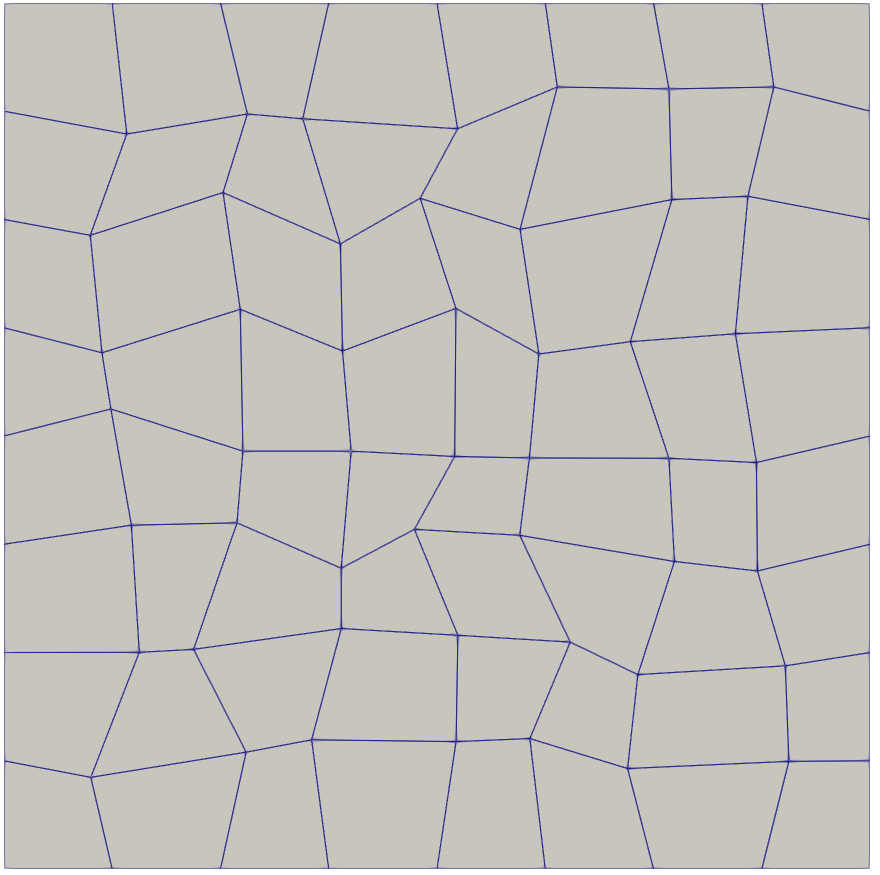
\includegraphics[width=\textwidth]{png/mesh_0.png}
  \end{subfigure}\qquad
  \hfill
  \begin{subfigure}[b]{0.28\textwidth}
    \centering
    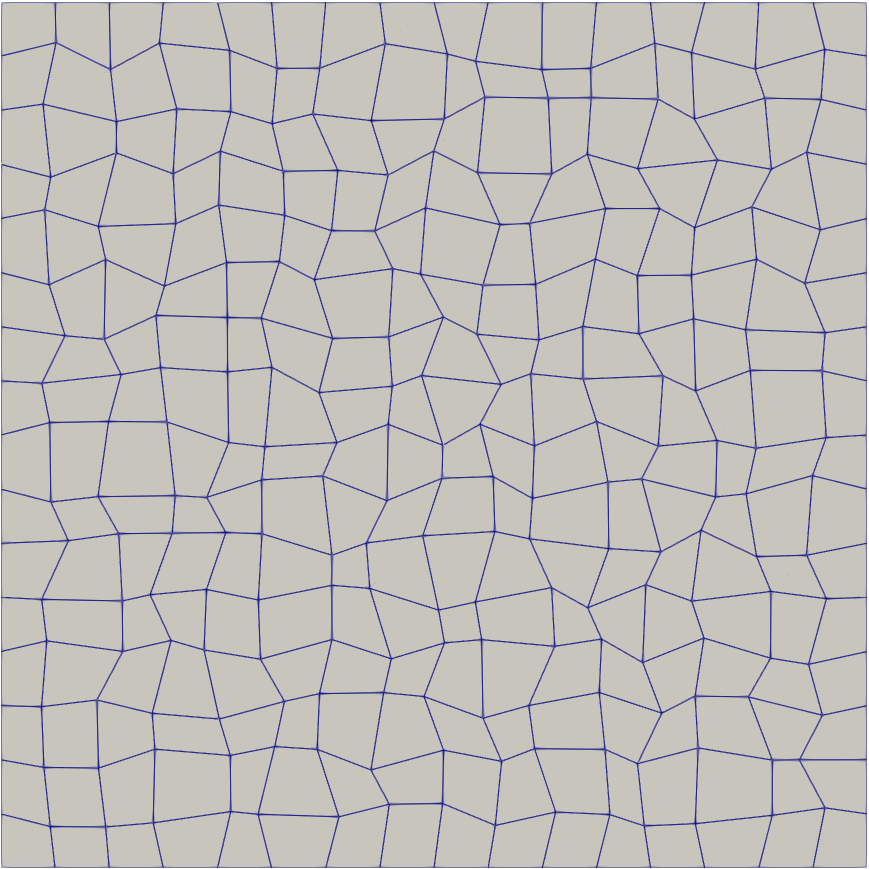
\includegraphics[width=\textwidth]{png/mesh_1.png}
  \end{subfigure}
  \hfill
  \begin{subfigure}[b]{0.28\textwidth}
    \centering
    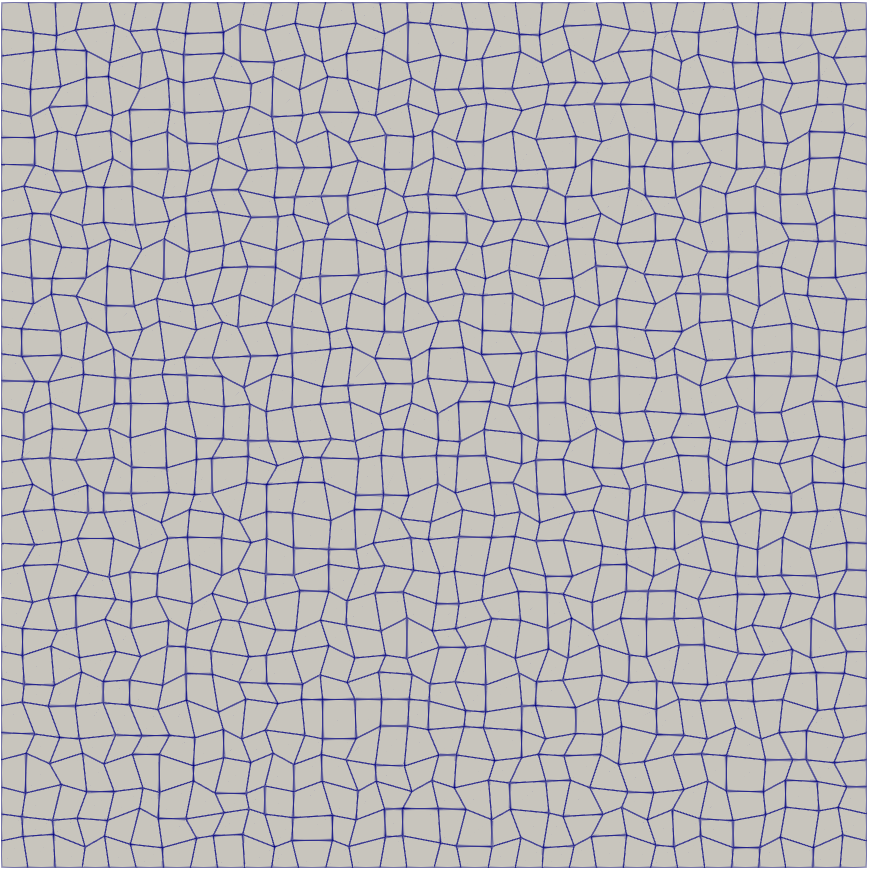
\includegraphics[width=\textwidth]{png/mesh_2.png}
  \end{subfigure}
  \caption{\it Example of non-nested multigrid levels.}\label{fig:nonnested}
\end{figure}

The current implementation extends the existing global-coarsening infrastructure by
introducing, in addition to the (conformal) \texttt{MGTwoLevelTransfer},
 a new (non-conformal) two-level transfer operator:
\begin{c++}
MGTwoLevelTransferNonNested two_level_transfer(/*...*/);

two_level_transfer.reinit(dof_handler_fine, dof_handler_coarse,
                          // the following parameters are optional
                          mapping_fine, mapping_coarse, 
                          constraints_fine, constraints_coarse)
\end{c++}
The resulting object can be passed to \texttt{MGTransferGlobalCoarsening} (and
\texttt{MGTransferBlockGlobalCoarsening}) in the usual way. The
interface of the new class is purposefully similar to
\texttt{MGTwoLevelTransfer},
with the difference that the former (i) also
takes \texttt{Mapping} instances, and (ii) is not limited to the case
that the coarser of the two \texttt{DoFHandler} instances can be generated by a coarsening step from the fine
mesh.

At the time of writing, the \texttt{MGTwoLevelTransferNonNested} operator provides a prolongation operator $\mathcal{P}^{(f,c)}$
that prolongates a vector $x^{(c)}$ from the coarse space to the fine space:
\begin{align*}
x^{(f)} = \mathcal{P}^{(f, c)}  x^{(c)},
\end{align*}
by a pointwise interpolation (injection) from the coarse mesh to the support points of the fine mesh. This is done
by looping over all coarse cells and interpolating to all (fine support) points that fall into the cell with
\texttt{FEPointEvaluation}. The local result is scattered into $x^{(f)}$, which is finalized by a
communication and a weighting step that is necessary as multiple elements could add to the same global entry.


The current implementation works for scalar and vectorial, continuous (\texttt{FE\_Q})
and discontinuous (\texttt{FE\_DGQ}) elements on hypercube-shaped cells. We plan to support
simplex elements and to add support
for projection, in addition to the pointwise interpolation outlined
above. Furthermore, we envision providing utility tools to generate
coarser 
meshes, based on a fine mesh. Currently, the users themselves 
have to provide such meshes,
e.g., by generating meshes with different cell sizes in external mesh-generation tools.

Note that the new class \texttt{MGTwoLevelTransferNonNested} is not limited to
multigrid but can be used to prolongate results and restrict residuals between any
two meshes. Indeed, the infrastructure has been successfully applied to perform
conservative interpolation between a fine (near) mesh and a coarse (far) mesh in the
context of aeroacoustic problems.
\todo{Can we add a reference for this?}


%%%%%%%%%%%%%%%%%%%%%%%%%%%%%%%%%%%%%%%%%%%%%%%%%%%%%%%%%%%%%%%%%%%%%%%%%%%%%%%%
\subsection{New linear algebra features}\label{sec:lac}

There are a number of linear-algebra related new features in this release:
\begin{itemize}
  \item Both \texttt{SolverGMRES} and \texttt{SolverFGMRES} now support the classical
  Gram--Schmidt orthonormalization in addition to the modified Gram--Schmidt algorithm. This
  reduces the cost of vector operations in terms of
  communication latency and memory transfer significantly.
  \item Our Chebyshev preconditioner (\texttt{PreconditionChebyshev}) now also
  supports James Lottes’s novel fourth-kind Chebyshev
  polynomial~\cite{lottes2022optimal, phillips2022optimal}.
  \item Our relaxation preconditioner (\texttt{PreconditionRelaxation}) now also
  allows interleaving cell loops and vector updates related to relaxation. The
  relaxation iteration reads as
  \begin{align*}
  x^{(i+1)} \gets x^{(i)} + \omega P^{-1}(b-Ax^{(i)}).
  \end{align*}
  In the case that the preconditioner $P$ is a diagonal matrix, the zeroing of
  the destination vector $x_{i+1}$ can be performed during a
  \texttt{pre}-operation  of the application of $A$
  and the vector update $x^{(i+1)}_j \gets x^{(i)}_j + \omega P^{-1}_{j,j}(b_j-(Ax^{(i)})_j)$
  during a \texttt{post} operation, allowing for a reduction in the number of read and write
  accesses from 8 and 4, to 1 and 3, respectively. The existing \texttt{pre}/\texttt{post}
  support in our Chebyshev-preconditioner implementation (\texttt{PreconditionChebyshev})
  has been improved. In addition, both \texttt{PreconditionRelaxation} and 
  \texttt{PreconditionChebyshev} support \texttt{pre}/\texttt{post} optimizations
  now not only for diagonal preconditioners but also for preconditioners that are
  built around cell loops and, as a consequence, support interleaving. Examples of
  such preconditioners are patch-based additive Schwarz preconditioners.
  \item In the context of additive Schwarz methods, the preconditioner application
  is defined as
  \begin{align*}
  v = P^{-1} u = \sum R_i^\top A_i^{-1} R_i u 
  \end{align*}
  with $A_i = R_i A R_i^T$ being a block of the assembled system
  matrix $A$ restricted
  to an index set described by $R_i$. In the special case when $R_i$ denotes the unknowns
  of cells, the expression $R_i A R_i^T$ resembles the reverse of matrix
  assembly.
  During the restriction step,
  rows of the system matrix that are potentially owned by other
  processes are needed.  In \dealii, it is not possible to access remote entries
  of sparse matrices. Two new functions query this information. First,
  \texttt{restrict\_to\_serial\_sparse\_matrix()} creates, based
  on a given index set, a serial
  sparse matrix from a distributed matrix:
\begin{c++}
SparseMatrixTools::restrict_to_serial_sparse_matrix (
  sparse_matrix_in, sparsity_pattern, requested_index_set, 
  system_matrix_out, sparsity_pattern_out)
\end{c++}
This function can be used, e.g., if the granularity of the additive Schwarz preconditioner
is a complete subdomain, potentially, with a fixed overlap.

In contrast, \texttt{restrict\_to\_full\_matrices()} performs the restriction
for arbitrary number of patches/blocks:

\begin{c++}
SparseMatrixTools::restrict_to_full_matrices (
  sparse_matrix_in, sparsity_pattern, indices_of_blocks, blocks)
\end{c++}

The data is stored in dense matrices, since the typical granularity is a (rather small) cell-centric or
vertex-star patch.
  
  \item For certain types of configurations, there are computationally more efficient
  approaches than extracting submatrices from an assembled matrix. For
  example, for the Laplace
  operator on 2D Cartesian meshes, the (element/patch) matrix is given as
  \begin{align*}
  A_i^{\text{cart}} = K_1 \otimes M_0 + M_1 \otimes K_0,
  \end{align*}
  i.e., as the tensor product of 1D mass and stiffness matrices. The inverse is
  explicitly available via the fast diagonalization method~\cite{lynch1964direct} as
  \begin{align*}
  \left(A_i^{\text{cart}}\right)^{-1} = (T_1 \otimes T_0) (\Lambda_1 \otimes I + I \otimes \Lambda_0)^{-1} (T_1^\top \otimes T_0^\top),
  \end{align*}
  with $T_i$ and $\Lambda_i$ being the (orthonormal) eigenvectors and the diagonal
  matrix of eigenvalues, obtained from a generalized eigendecomposition
  $K_iT_i =  M_i T_i \Lambda_i$, as also used by \dealii's \texttt{step-59} tutorial program.
  Since $A_i \approx A_i^{\text{cart}}$
  might be a good approximation also in the case of non-Cartesian meshes and 
  $A_i^{\text{cart}}$ has an explicit inverse, it is considered in the
  literature as a patch preconditioner in the context of additive
  Schwarz~\cite{witte2021fast, phillips2021auto, couzy1995spectral} and block-Jacobi methods~\cite{kronbichler2019hermite}.
  In \dealii, the new function
  \texttt{Tensor\-Product\-Matrix\-Creator::create\_\allowbreak laplace\_\allowbreak tensor\_\allowbreak product\_\allowbreak matrix()} computes $K_i$ and $M_i$
  for cell-centric patches with a specified overlap and given boundary conditions.
  A set of $T_i$ and $\Lambda_i$ is applied to a cell via
  \texttt{Tensor\-Product\-Matrix\-Symmetric\-Sum} or to a collection of cells
  via the new class \texttt{Tensor\-Product\-Matrix\-Symmetric\-Sum\-Collection}, which
  tries to reuse the eigenvalues and eigenvectors between cells.
\end{itemize}


%%%%%%%%%%%%%%%%%%%%%%%%%%%%%%%%%%%%%%%%%%%%%%%%%%%%%%%%%%%%%%%%%%%%%%%%%%%%%%%%
\subsection{C++ language modernization}\label{sec:language}

\dealii{} currently uses C++14 as the language standard to which its
code base is written. It can also use the classes
\texttt{std::optional} and \texttt{std::variant} if the compiler
supports C++17, but falls back to implementations obtained via the
BOOST library otherwise, and this is true also for a number of
individual functions that were introduced in C++17 or C++20.

As part of the current release, \dealii{} now also uses some C++20
features to annotate classes and functions with regard to properties
template arguments need to satisfy. This aids in situations such as
with the
following function:
\begin{c++}
  template <class MeshType>
  std::vector<typename MeshType::active_cell_iterator>
  find_cells_adjacent_to_vertex(const MeshType &   mesh,
                                const unsigned int vertex);
\end{c++}
This function is intended to be called with either a
\texttt{Triangulation} or \texttt{DoFHandler} object as first
argument (and documents this requirement), but the compiler can not check this requirement at the call
site and will gladly call it with any other kind of object as
well. Because the implementation of the function is in a \texttt{.cc}
file, and the template is only instantiated for the two classes
mentioned above, calling the function (erroneously) with anything else
as first argument is not detected at compile time, but only later when
the linker reports an undefined symbol.

We have started to address this by annotating functions using
C++20-style ``\texttt{requires}'' clauses:
\begin{c++}
  template <class MeshType>
    requires (concepts::is_triangulation_or_dof_handler<MeshType>)
  std::vector<typename MeshType::active_cell_iterator>
  find_cells_adjacent_to_vertex(const MeshType &   mesh,
                                const unsigned int vertex)
\end{c++}
If the compiler supports C++20, then the added clause will cause the
compiler to reject any call to the function for which the first
argument \texttt{MeshType} does not satisfy the named concept, which
is internally defined as the type being either a \texttt{Triangulation} or \texttt{DoFHandler}
object, as intended. (The \texttt{requires} annotation is suppressed if the compiler
does not support C++20.)

Given the heavy dependence of \dealii{} on templates, there are likely
hundreds or thousands of locations that should be annotated with
requirements on template arguments over time; for the moment, the
library contains some 300 of these \texttt{requires} clauses.


%%%%%%%%%%%%%%%%%%%%%%%%%%%%%%%%%%%%%%%%%%%%%%%%%%%%%%%%%%%%%%%%%%%%%%%%%%%%%%%%
\subsection{Build-system modernization}\label{sec:buildsystem}

\todo[inline]{Write}


%%%%%%%%%%%%%%%%%%%%%%%%%%%%%%%%%%%%%%%%%%%%%%%%%%%%%%%%%%%%%%%%%%%%%%%%%%%%%%%%
\subsection{New and improved tutorials and code gallery programs}
\label{subsec:steps}

While there are no new \dealii tutorial programs in this release, many
were extensively revised: Around 130 of the more than 2000 (non-merge)
commits that went into this release touched the tutorial, in some
cases adding substantial amounts of text.

% data generated using these commands:
% - tutorial: git log --since 2022/06/01 --no-merges examples | grep commit | wc -l
% - total:    git log --since 2022/06/01 --no-merges | grep commit | wc -l

There are also three new programs in the code gallery (a collection of
user-contributed programs that often solve more complicated problems
than tutorial programs, and that are intended as starting points for further
research rather than as teaching tools):
\begin{itemize}
  \item \textit{``A posteriori error estimator for first order hyperbolic problems''},
  contributed by Marco Feder;
  \item \textit{``Distributed moving laser heating''}, contributed by
  Hongfeng Ma and Tatiana E.~Itina;
  \item \textit{``Generalized Swift-Hohenberg Equation Solver''}, contributed by
  Sam Scheuerman.
\end{itemize}


%%%%%%%%%%%%%%%%%%%%%%%%%%%%%%%%%%%%%%%%%%%%%%%%%%%%%%%%%%%%%%%%%%%%%%%%%%%%%%%%
\subsection{Incompatible changes}\label{subsec:deprecated}

The 9.5 release includes
\href{https://dealii.org/developer/doxygen/deal.II/changes_between_9_4_2_and_9_5_0.html}
{around X incompatible changes}; see \cite{changes95}. Many of the
incompatible change internal
interfaces that are not usually used in external
applications. That said, the following are worth mentioning since they
may have been more widely used:
\begin{itemize}
  \item
  The class \texttt{hp::DoFHandler} has been removed. The
  \texttt{DoFHandler} class now implements all $hp$-related
  functionality, as it has for the past few releases.

  \item
  We improved the type safety for active and future FE indices in the \texttt{DoFHandler} implementation by introducing a new data type \texttt{types::fe\textunderscore{}index}. Corresponding functions like \texttt{DoFCellAccessor::active\textunderscore{}fe\textunderscore{}index()} and \texttt{DoFHandler::get\textunderscore{}active\textunderscore{}fe\textunderscore{}indices()} have changed their interface.

  \item
  This rework also affects the serialization process of active FE indices. You will need to recreate your serialized data \textit{if and only if} you work in $hp$-mode. You can continue to use previously generated data if you do not use $hp$-mode. A special case forms \texttt{parallel::distributed::Triangulation} for non-$hp$ data, in which it is sufficient to increase the version in the metadata file by one from ``4'' to ``5''.

\item Several old interfaces to \texttt{MatrixFree} have been removed, e.g.,
  initialization functions without \texttt{Mapping} argument, the query
  to the number of cell batches, \texttt{DoFHandler} objects. In
  each case, new interfaces are available.

\item
  ...
\end{itemize}
\todo[inline]{Write}



%%%%%%%%%%%%%%%%%%%%%%%%%%%%%%%%%%%%%%%%%%%%%%%%%%%%%%%%%%%%%%%%%%%%%%%%%%%%%%%%
%%%%%%%%%%%%%%%%%%%%%%%%%%%%%%%%%%%%%%%%%%%%%%%%%%%%%%%%%%%%%%%%%%%%%%%%%%%%%%%%
%%%%%%%%%%%%%%%%%%%%%%%%%%%%%%%%%%%%%%%%%%%%%%%%%%%%%%%%%%%%%%%%%%%%%%%%%%%%%%%%
\section{How to cite \dealii}\label{sec:cite}

In order to justify the work the developers of \dealii put into this
software, we ask that papers using the library reference one of the
\dealii papers. This helps us justify the effort we put into this library.

There are various ways to reference \dealii. To acknowledge the use of
the current version of the library, \textbf{please reference the present
  document}. For up-to-date information and a bibtex entry
see
\begin{center}
  \url{https://www.dealii.org/publications.html}
\end{center}

The original \dealii paper containing an overview of its
architecture is \cite{BangerthHartmannKanschat2007}, and a more recent
publication documenting \dealii's design decisions is available as \cite{dealII2020design}. If you rely on
specific features of the library, please consider citing any of the
following:
\begin{multicols}{2}
  \vspace*{-36pt}
  \begin{itemize}[leftmargin=4mm]
    \item For geometric multigrid: \cite{Kanschat2004,JanssenKanschat2011,ClevengerHeisterKanschatKronbichler2019, munch2022gc};
    \item For distributed parallel computing: \cite{BangerthBursteddeHeisterKronbichler11};
    \item For $hp$-adaptivity: \cite{BangerthKayserHerold2007,fehling2022};
    \item For partition-of-unity (PUM) and finite element enrichment methods:
           \cite{Davydov2016};
    \item For matrix-free and fast assembly techniques:
          \cite{KronbichlerKormann2012,KronbichlerKormann2019};
    \item For computations on lower-dimensional manifolds:
          \cite{DeSimoneHeltaiManigrasso2009};
    \item For curved geometry representations and manifolds:
          \cite{HeltaiBangerthKronbichlerMola2019};
    \item For integration with CAD files and tools:
          \cite{HeltaiMola2015};
    \item For boundary element computations:
          \cite{GiulianiMolaHeltai-2018-a};
    \item For the \texttt{LinearOperator} and
      \texttt{Packaged\-Operation} facilities:
          \cite{MaierBardelloniHeltai-2016-a,MaierBardelloniHeltai-2016-b};
    \item For uses of the \texttt{WorkStream} interface:
          \cite{TKB16};
    \item For uses of the \texttt{ParameterAcceptor} concept, the
          \texttt{MeshWorker::ScratchData} base class, and the
          \texttt{ParsedConvergenceTable} class:
          \cite{SartoriGiulianiBardelloni-2018-a};
    \item For uses of the particle functionality in \dealii:
          \cite{GLHPB18}.
          \vfill\null
  \end{itemize}
\end{multicols}

\dealii can interface with many other libraries:
\begin{multicols}{3}
  \begin{itemize}[leftmargin=4mm]
    \item ADOL-C \cite{griewank1996adolc}
    \item ArborX \cite{lebrun2020arborx}
    \item ARPACK \cite{lehoucq1998arpack}
    \item Assimp \cite{schulze2021assimp}
    \item BLAS and LAPACK \cite{anderson1999lapack}
    \item Boost \cite{boost-web-page}
    \item CGAL \cite{cgal-user-ref}
    \item cuSOLVER \cite{cusolver-web-page}
    \item cuSPARSE \cite{cusparse-web-page}
    \item Gmsh \cite{geuzaine2009gmsh}
    \item GSL \cite{galassi2009gsl,gsl-web-page}
    \item Ginkgo \cite{anzt2020ginkgo,anzt2022ginkgo}
    \item HDF5 \cite{hdf5-web-page}
    \item METIS \cite{karypis1998metis}
    \item MUMPS \cite{amestoy2001mumps,amestoy2019mumps}
    \item muparser \cite{muparser-web-page}
    \item OpenCASCADE \cite{opencascade-web-page}
    \item p4est \cite{burstedde2011p4est,burstedde2020parallel}
    \item PETSc \cite{petsc-user-ref,petsc-web-page}
    \item ROL \cite{ridzal2014rol}
      \todo{ROL is part of Trilinos. Do we also need to cite something
        for NOX?}
    \item ScaLAPACK \cite{blackford1997scalapack}
    \item SLEPc \cite{hernandez2005slepc}
    \item SUNDIALS \cite{hindmarsh2005sundials}
    \item SymEngine \cite{symengine-web-page}
    \item TBB \cite{reinders2007tbb}
    \item Trilinos \cite{heroux2005trilinos,trilinos-web-page}
    \item UMFPACK \cite{davis2004umfpack}
  \end{itemize}
\end{multicols}
Please consider citing the appropriate references if you use
interfaces to these libraries.

The two previous releases of \dealii can be cited as
\cite{dealII92,dealII93}.


\section{Acknowledgments}

\dealii is a worldwide project with dozens of contributors around the
globe. Other than the authors of this paper, the following people
contributed code to this release:\\
%
% Uwe Koecher doesn't usually show up in the changelog, but
% we should make sure he's listed.
%

% This is up-to-date as of 9.4 RC1 - should be the final list.

\todo[inline]{Add.}


Their contributions are much appreciated!


\bigskip

\dealii and its developers are financially supported through a
variety of funding sources:

\todo[inline]{Need to update. Also remove those not on the current paper.}

D.~Arndt and B.~Turcksin: Research sponsored by the Laboratory Directed Research and
Development Program of Oak Ridge National Laboratory, managed by UT-Battelle,
LLC, for the U. S. Department of Energy.

W.~Bangerth and T.~Heister were partially
supported by the Computational Infrastructure for Geodynamics initiative
(CIG), through the National Science Foundation (NSF) under Award
No.~EAR-1550901 and The University of California -- Davis.
\todo{This is the CIG-II grant. We need to update this to the CIG-III
  (and CIG-IV?) grants.}

W.~Bangerth and M.~Fehling were partially supported by Award OAC-1835673
as part of the Cyberinfrastructure for Sustained Scientific Innovation (CSSI)
program.

W.~Bangerth was also partially supported by Awards DMS-1821210 and EAR-1925595.

M.~Bergbauer was supported by the German Research Foundation (DFG) under the
project ``High-Performance Cut Discontinuous Galerkin Methods for Flow
Problems and Surface-Coupled Multiphysics Problems'' Grant Agreement
No.~456365667.

J.~Heinz was supported by the European Union’s Framework Programme for Research
and Innovation Horizon 2020 (2014-2020) under the Marie Sk\l{}odowska--Curie Grant
Agreement No. [812719].

T.~Heister was also partially supported by NSF
Awards OAC-2015848, DMS-2028346, and
EAR-1925575.

L.~Heltai was partially supported by the Italian Ministry of Instruction,
University and Research (MIUR), under the 2017 PRIN project NA-FROM-PDEs MIUR
PE1, ``Numerical Analysis for Full and Reduced Order Methods for the efficient
and accurate solution of complex systems governed by Partial Differential
Equations''.

M.~Kronbichler and P.~Munch were partially supported by the
German Ministry of Education and Research, project
``PDExa: Optimized software methods for solving partial differential
equations on exascale supercomputers'' and the Bayerisches Kompetenznetzwerk
f\"ur Technisch-Wissen\-schaft\-li\-ches Hoch- und H\"ochstleistungsrechnen
(KONWIHR), projects ``High-order matrix-free finite
element implementations with hybrid parallelization and improved data
locality'' and ``Fast and scalable finite element algorithms for coupled
multiphysics problems and non-matching grids''.

M.~Maier was partially supported by NSF Award DMS-2045636 and and by the
Air Force Office of Scientific Research under grant/contract number
FA9550-23-1-0007.

D.~Wells was supported by the NSF Award OAC-1931516.

\bibliography{paper}{}
\bibliographystyle{abbrv}

\end{document}
